\documentclass[a0,portrait]{a0poster}

\usepackage{multicol} % This is so we can have multiple columns of text side-by-side
\columnsep=100pt % This is the amount of white space between the columns in the poster
\columnseprule=3pt % This is the thickness of the black line between the columns in the poster

\usepackage[svgnames]{xcolor} % Specify colors by their 'svgnames', for a full list of all colors available see here: http://www.latextemplates.com/svgnames-colors

\usepackage{times} % Use the times font
%\usepackage{palatino} % Uncomment to use the Palatino font

\usepackage{graphicx} % Required for including images
\usepackage{wrapfig}
\graphicspath{{figures/}} % Location of the graphics files
\usepackage{booktabs} % Top and bottom rules for table
\usepackage[font=small,labelfont=bf]{caption} % Required for specifying captions to tables and figures
\usepackage{amsfonts, amsmath, amsthm, amssymb} % For math fonts, symbols and environments
\usepackage{wrapfig} % Allows wrapping text around tables and figures

\newcommand{\Sta}{y}
\newcommand{\Adj}{p}
\newcommand{\Con}{u}

\begin{document}
\thispagestyle{empty}
\vspace{-5cm}
\title{\veryHuge \color{NavyBlue} \textbf{PDE-Constrained Optimization for Multiscale Particle Dynamics} \color{Black}} % Title
\author{}
\date{}
\maketitle
\vspace{-4cm}
\begin{minipage}[b]{0.65\linewidth}
\Huge{With Industrial Applications}\\[1cm] % Subtitle
\huge \textbf{Jonna Roden}\\[0.5cm] % Author(s)
\huge University of Edinburgh, MIGSAA\\[0.4cm] % University/organization
\Large {Supervision by Dr Ben Goddard and Dr John Pearson} \\
\end{minipage}
\begin{minipage}[b]{0.35\linewidth}
	\vspace{-7cm}

\includegraphics[width=7cm]{EdinburghUni.png} \ \ \ \ \ \ \ \ \ \ 
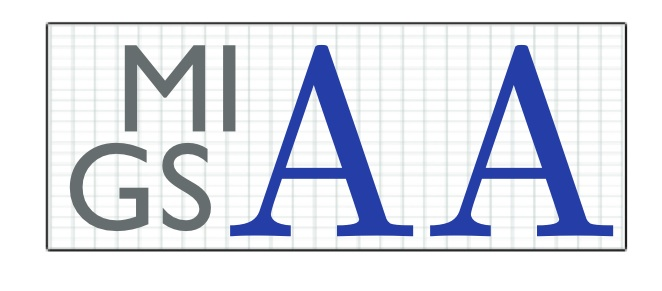
\includegraphics[width=15cm]{MIGSAA.jpg}\\
\vspace{1cm}
\end{minipage}

\vspace{-1cm} % A bit of extra whitespace between the header and poster content

%----------------------------------------------------------------------------------------

\begin{multicols}{2} % This is how many columns your poster will be broken into, a portrait poster is generally split into 2 columns

%----------------------------------------------------------------------------------------
%	ABSTRACT
%----------------------------------------------------------------------------------------

%\color{Navy} % Navy color for the abstract



%----------------------------------------------------------------------------------------
%	INTRODUCTION
%----------------------------------------------------------------------------------------

%\color{DarkSlateGray}

\section*{Introduction}
There are many industrial processes that can be described by the integro-PDEs for multiscale particle dynamics and optimized using PDE-constrained optimization techniques. An example of such an industrial problem is minimizing the sedimentation time of yeast particles in beer to optimize the brewing process. The industrial partners of the PhD project are WEST Beer and uFraction8. Solving PDE-constrained optimization problems involving integro-PDE-constraints requires the development of new theoretical and numerical methods, which is addressed in this work. 

%\color{DarkSlateGray}
\section*{Multiscale Particle Dynamics}
The dynamics of the particle density $\Sta$ at position $x$ and time $t$ can be described by the PDE, see \cite{RexLoewen1}:
\begin{align*}
\partial_t \Sta(x,t) &=\nabla^2 \Sta(x,t) +u (x,t)+\alpha \nabla \cdot\int_\Omega \Sta(x,t) \Sta(x',t) \nabla V_2(|x-x'|)dx',\qquad \ \ \ \ \ \text{in   } \ \ \quad \Omega \times (0,T),\\
\frac{\partial \Sta(x,t)}{\partial n} &+\int_\Omega \Sta(x,t) \Sta(x',t) \frac{\partial V_2(x)}{\partial n}dx'=0, \quad \qquad\qquad\qquad\qquad\qquad\qquad\qquad  \text{on   } \quad \partial \Omega \times (0,T),\\
\\
\Sta(x,0) &=\Sta_0(x).
\end{align*}
 The natural boundary condition for this problem is no-flux. However, other boundary conditions can be imposed, such as Dirichlet boundary conditions (used in Figure \ref{Result1}).
%\color{DarkSlateGray} % DarkSlateGray color for the rest of the content

\section*{Optimal Control Problem}
One PDE-constrained optimization problem involving the above particle dynamics is:
\begin{align*}
&\min_{\Sta,u} \quad \frac{1}{2}||{\Sta(x,t)- \hat{\Sta}(x,t)}||_{L_2(\Omega \times [0,T])}^2 + \frac{\beta}{2} ||{\Con}(x,t)||_{L_2(\Omega \times [0,T])}^2\\
\\
&\text{subject to:}
\\
&\partial_t \Sta(x,t) =\nabla^2 \Sta(x,t) +\Con(x,t) + \alpha \nabla \cdot\int_\Omega \Sta(x,t) \Sta(x',t) \nabla V_2(|x-x'|)dx' \\
&+\text{BCs} + \text{ICs for } \Sta.
\end{align*}
 In this example, the forcing term $\Con$ in the PDE is the control variable. However, the control can be enforced in other ways, e.g. through boundary conditions.
\section*{First Order Optimality System}
 The first order optimality system for the above optimal control problem can be reduced to two coupled PDEs, that can be solved numerically: 
\begin{align*}
\text{Forward Problem}\\
\partial_t \Sta(x,t) &= \Delta \Sta(x,t) + \frac{1}{\beta}\Adj(x,t) +\alpha\int_\Omega\Sta(x,t) \Sta(x',t) \nabla_x V_2(|x-x'|)dx',\\
\text{Adjoint Equation}\\
\partial_t \Adj(x,\tau) &=  \Delta \Adj(x,\tau) -\Sta(x,\tau) +\hat{\Sta}(x,\tau) \phantom{\int} \\
&+\alpha\int_\Omega \bigg( \nabla_x \Adj(x,\tau) + \nabla_{x'} \Adj(x',\tau) \bigg) \Sta(x',\tau) \nabla_x V_2(|x-x'|)dx',\\
+\text{BCs} + &\text{ICs for } \Sta(x,t) \text{ and } \Adj(x,\tau).
\end{align*}
The Adjoint Equation is running backward in time, with $\tau = T+t_0 -t$, for numerical stability.
\section*{Numerical Methods}
	\begin{wrapfigure}{r}{12cm}
	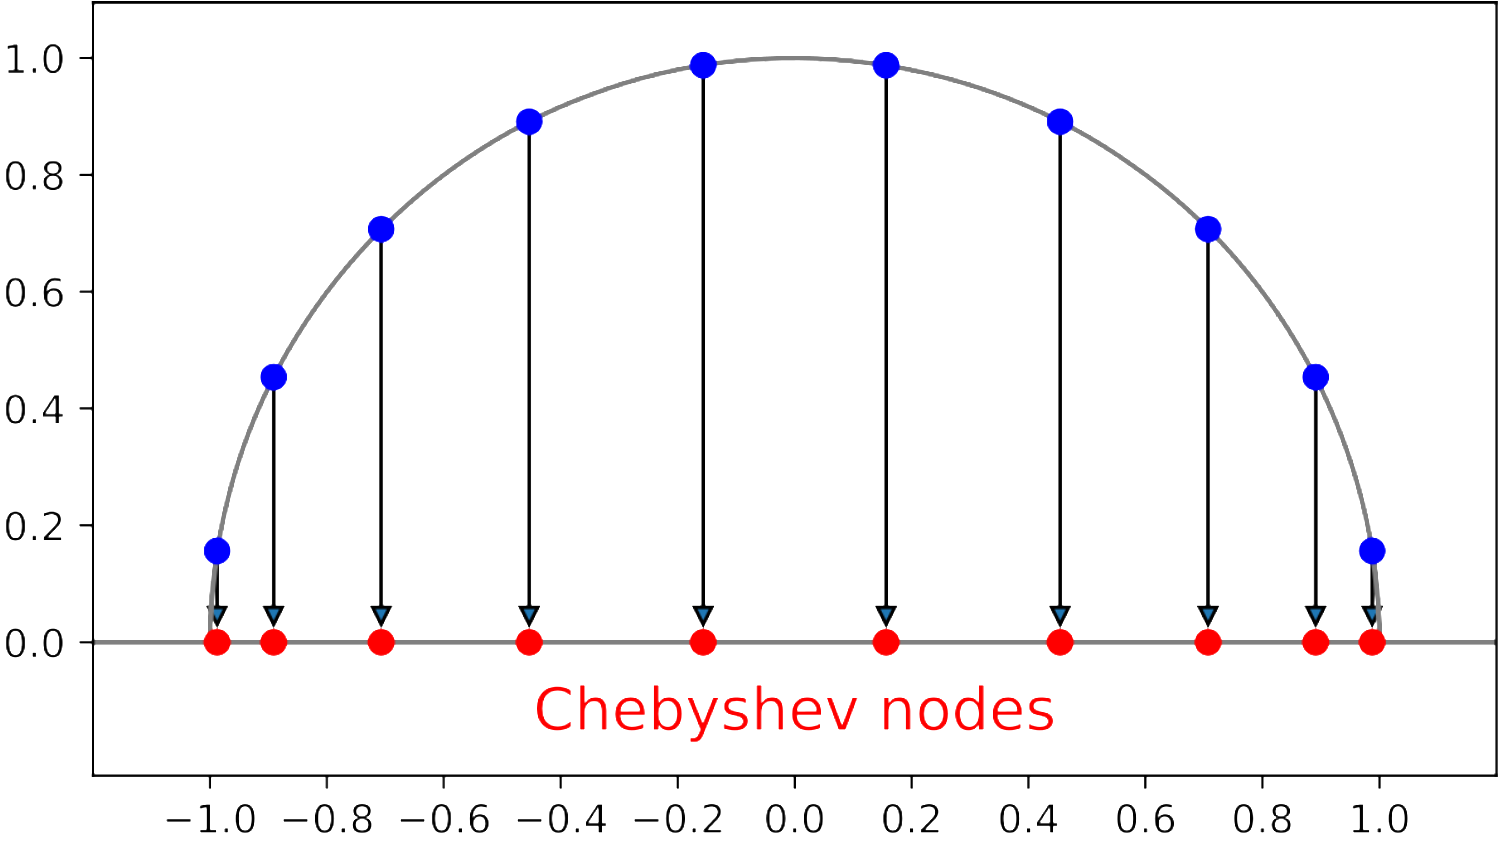
\includegraphics[width=12cm]{chebnodes1.png}
	\caption{\color{Blue} Chebyshev Points on $[-1,1]$}
	\label{Cheb}
\end{wrapfigure}
New approaches to solving the optimality system are needed because of the non-linear, non-local nature of the particle interaction term in the PDE-constraint. Additionally, the boundary conditions are non-local and problem specific. Moreover, due to the final time condition in the adjoint equation, the problem is a boundary value problem in time as well as in space. For these reasons, standard methods are no longer sufficient to solve this type of problem. 

\subsection*{Pseudospectral Methods} 

Pseudospectral methods on non-periodic domains are based on polynomial interpolation on non-equispaced points.   

\begin{itemize}

	\item
	
Collocation points: Chebyshev points $\{x_j\}$ on $[-1,1]$, defined as \cite{bibTrefethen}, see Figure \ref{Cheb}:

\begin{align*}
x_j= \cos\bigg(\frac{j \pi}{N}\bigg), \quad j=0,1,...,N.
\end{align*}	


\item

Interpolation: Barycentric Lagrange interpolation, derived in \cite{bibTrefethenBerrut1}.
\item 
Differentiation: Chebyshev differentiation matrices, see \cite{bibTrefethen}.
\item
Integration: Clenshaw--Curtis quadrature, derived in \cite{ClenCurt1}.
\item 
Advantages of pseudospectral methods: Can apply non-local boundary conditions easily, exponential convergence for smooth functions, see \cite{Boyd1}:
\begin{align*}
\text{Pseudospectral Error} \approxeq O \bigg[ \bigg( \frac{1}{N} \bigg)^N \bigg].
\end{align*}
\item  
Disadvantages of pseudospectral methods: complex domains are challenging to deal with, method involves (small) dense matrices. 
\end{itemize} 


\subsection*{Multiple Shooting Method \cite{CarraroIndMultipleShooting}}
\begin{itemize}
	\item Discretize the time interval into subintervals $[t_i,t_{i+1}]$.
	\item Create initial guesses for $\Sta$ and $\Adj$ at each $t_i$.
	\item Solve the PDEs on the subintervals.
	\item Interpolate $\Sta$ and $\Adj$ between $t_i$ and $t_{i+1}$ when necessary.
	\item Match the \textcolor{Red}{PDE solution} to the \textcolor{Blue}{initial guess} for $\Sta$ and $\Adj$ at each $t_i$ by optimizing the initial guess.
\end{itemize}
\begin{center}
	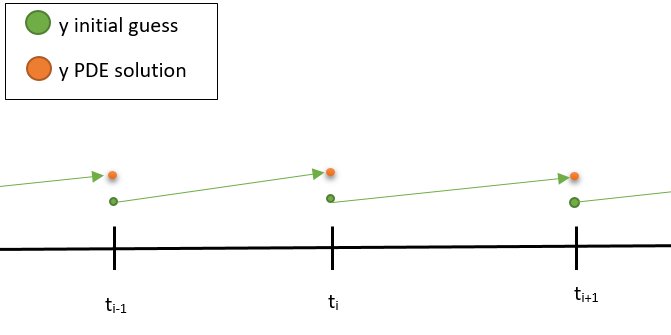
\includegraphics[width=17cm]{rhoSol.png}
	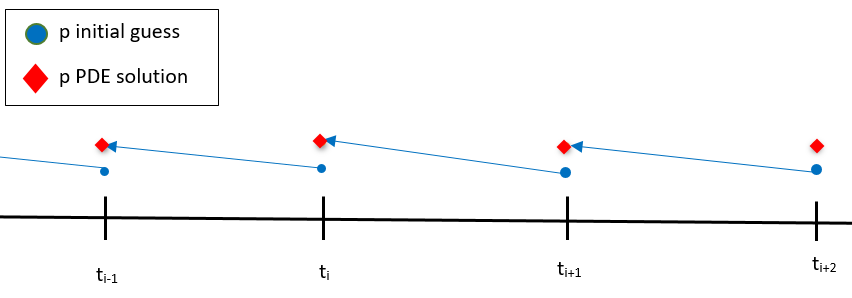
\includegraphics[width=17cm]{qSol.png}
	\captionof{figure}{\color{Blue} Multiple Shooting for $\Sta$ and $\Adj$.}
\end{center}
\section*{Results}
The optimality system can be solved using the multiple shooting approach and pseudospectral methods in time and space. The evolution of $\Sta$ and $\Adj$ are displayed in Figure \ref{Result1}, where each red dashed line represents a time step $t_i$, decreasing from the initial distribution at time $t=0$ to the target at time $T$. When $\alpha >0$, the particles are interacting repulsively and the particles spread more than when $\alpha=0$ and the particles are non-interacting. Note that in this example Dirichlet boundary conditions are imposed.

\begin{center}
		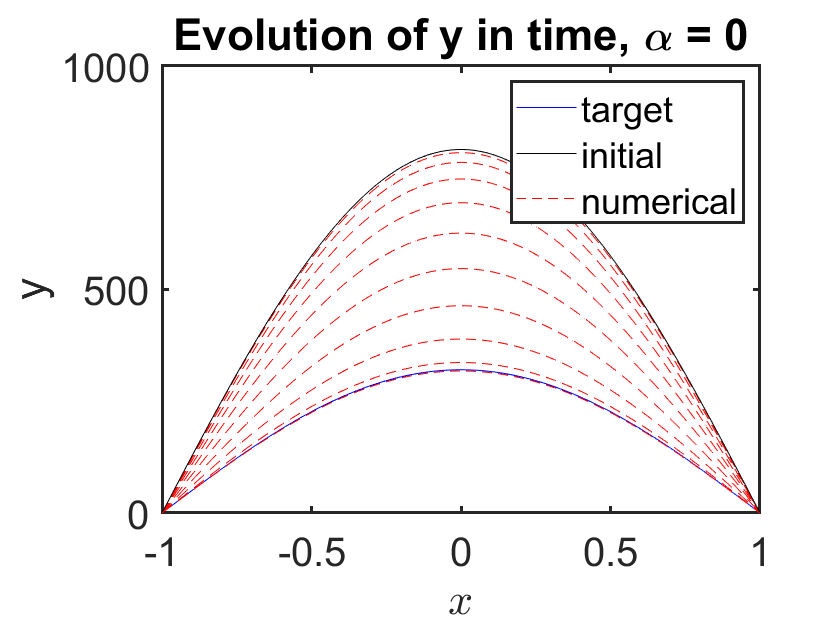
\includegraphics[scale=0.75]{Rhoalpha0.png}
		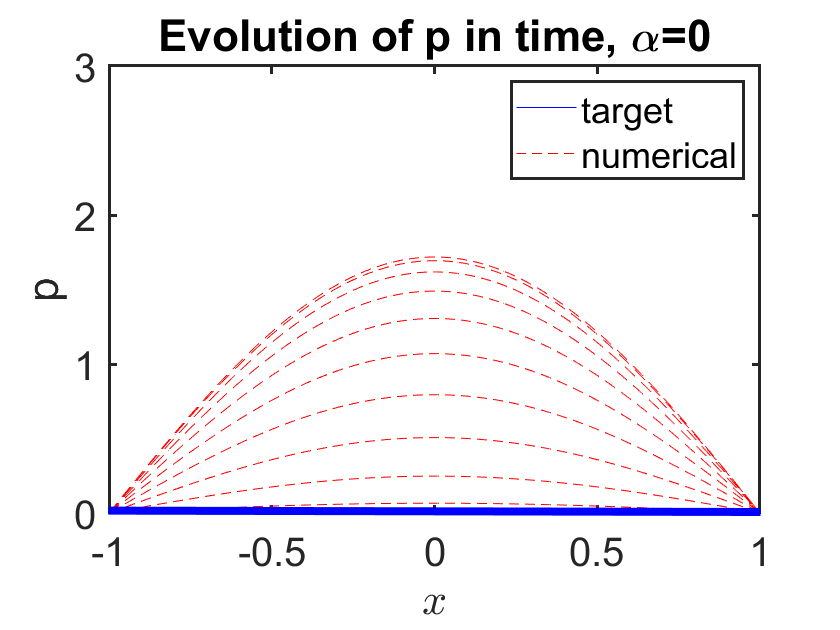
\includegraphics[scale=0.75]{qalpha0.png}
		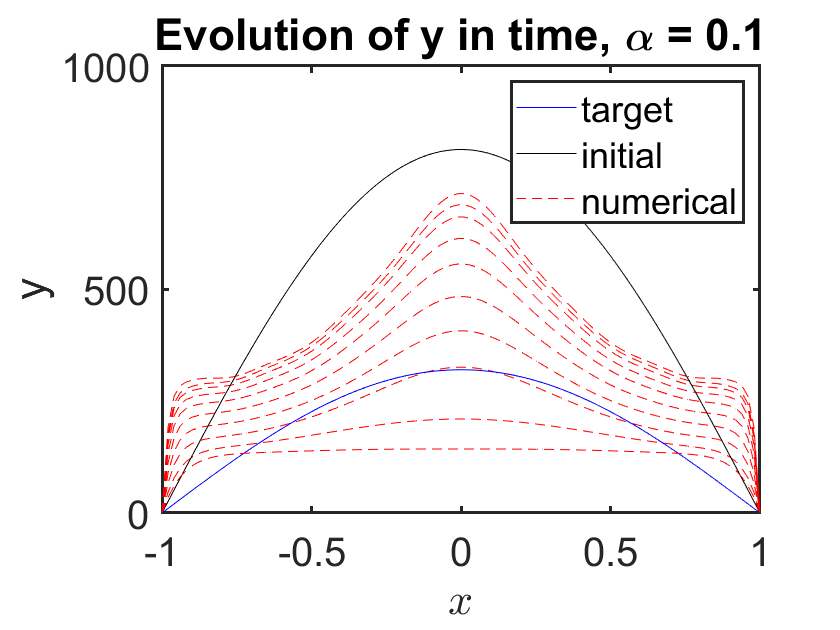
\includegraphics[scale=0.75]{Rhoalpha01.png}
		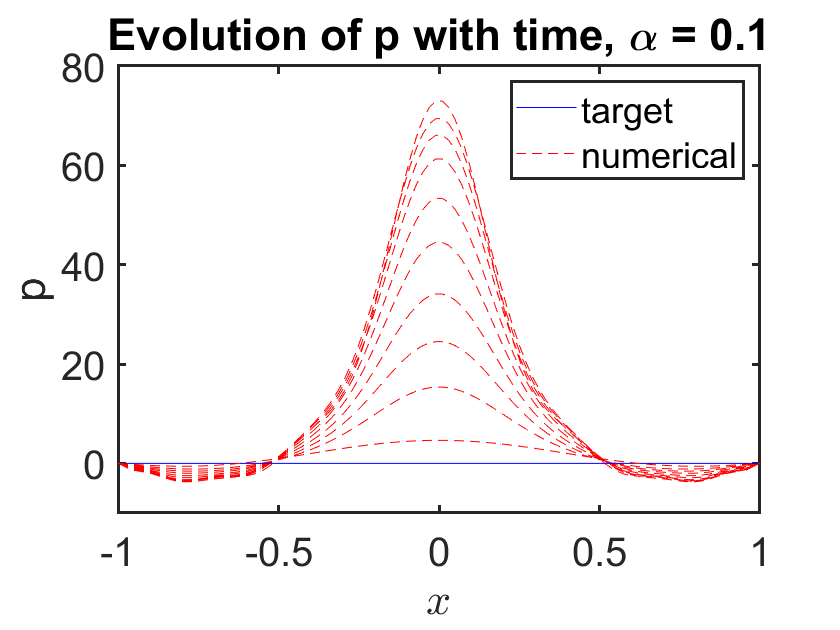
\includegraphics[scale=0.75]{qalpha01.png}
	%	\caption{Solution to the optimality system with $\alpha=0$ (top) and $\alpha=0.1$ (bottom), where $N=20$, $n=11$.}
		\vspace{-10pt}
\captionof{figure}{\color{Blue} Solution to the optimality system without ($\alpha=0$) and with ($\alpha>0$) particle interaction term. Each red dashed line indicates a time step moving from the initial distribution at time $t=0$ to the target distribution at time $T$.}
\label{Result1}
\end{center}

\section*{Forthcoming Research}

In the future, the existing code library (2DChebClass) \cite{GoddardPseudospectralCode1} will be extended to compute a wide range of PDE-constrained optimization problems for multiscale particle dynamics involving non-linear, non-local terms in one and two dimensions. 
The numerical method will be applied to industrial problems that aim at optimizing processes involving particle dynamics, such as nano filtration and sedimentation of yeast in beer.
For more information on the applications of this method, please see the poster by Mildred Aduamoah.
\thispagestyle{empty}
\bibliography{JonnaPosterBib}
\bibliographystyle{unsrt}


\end{multicols}
\end{document}